\documentclass{article}
\usepackage[utf8]{inputenc}
\usepackage{ffcode}
\usepackage{pgfplots}
\pgfplotsset{width=8cm,compat=1.9}

\def\dunderline#1{\underline{\underline{#1}}}

\title{Algoritmer og Datastrukturer Øving 2}
\author{Nicolai H. Brand}
\date{September 2022}

\begin{document}

\maketitle

Kompiler og kjør programmet kan gjøres ved:
\begin{ffcode}
cc oblig2.c -lm && ./a.out
\end{ffcode}

\section{Asymptotisk analyse}

Tidskomplesiten til en rekursive algoritme kan beskrives med

$ T(n) = aT(n/b) + cn^k $

Hvor \(a\) er antall rekursive kall i funcksjonen, \(b\) er brøkdelen av datasettet vi behandler i et rekursivt tall, og \(cn^k\) er vanlige løkker

\subsection{Asymptotisk analyse av 2.1-1}
\begin{ffcode}
double my_pow1(double x, int n)
{
    if (n == 0)
        return 1;
        
    return x * my_pow1(x, --n);
}
\end{ffcode}

Funksjonen blir kalt \(1\) ganger per kall som gir \(a = 1\). Datasettet minker med \(n - 1\) for hvert kall til funksjonen. Det er en if-setning, men ingen løkker i algoritmen som vil si at \(k = 0\).\\\\
Dermed får vi:

$ \dunderline{T(n) = T(n - 1) + 1 \in \Theta(n)} $\\

\subsection{Asymptotisk analyse av 2.2-3}
\begin{ffcode}
double my_pow2(double x, int n)
{
    if (n == 0)
        return 1;
    
    if (n % 2 == 0)
        return my_pow2(x * x, n / 2);
        
    return x * my_pow2(x * x, (n - 1) / 2);
}
\end{ffcode}

I likhet med \textbf{2.2-3} kaller funksjonen seg selv \(1\) gang per kall, foruten basistilfellet. Derimot halveres datasettet for hvert kall til funksjonen. I likhet med \textbf{2.3-3} er det ingen løkker.\\\\
Dermed får vi:

$ T(n) = T(n / 2) + 1 $\\\\
Ser at \(b^k = 2^0 = 1\) som betyr \(b^k = a\)\\

Dermed blir \(T(n) \in \Theta(n^k{\log n})\)\\

Altså:\\

$ \dunderline{T(n) \in \Theta({\log n})} $


\section{Resultater}

Tabellen under viser hvor lang tid algoritmene skrevet i oppgave 1, 2, i tilleg til glibc sin implementasjon av \textbf{pow} brukte. I alle tilfellene ble \(x=1.001\) brukt, men n (eksponenten) varierer. Algoritmene ble kjørt 1000 ganger for å få et bedre gjennomsnitt. Dermed viser tiden hvor lang tid 1000 iterasjoner av algoritmen tar for en gitt eksponent \(n\).

\begin{center}
\begin{tabular}{|c c c c|} 
 \hline
 eksponent & 2.1-1 (s) & 2.2-3 (s) & glibc pow (s) \\ [0.5ex] 
 \hline\hline
 100 & 0.000875 & 0.000051 & 0.000014 \\ 
 \hline
 1.000 & 0.008804 & 0.000066 & 0.000010 \\
 \hline
 10.000 & 0.091680 & 0.000095 & 0.000014 \\
 \hline
 100.000 & 0.920433 & 0.000112 & 0.000010 \\
 
 \hline
\end{tabular}
\end{center}

\section{Diskusjon}

Med bakgrunn i resultatene er den umiddelbare observasjonen at algoritmen fra oppgave \textbf{2.1-1} er atskillelig tregere enn de to andre. Mer undersøkelse viser at når eksponenten \(n\) dobler, dobler også kjøretiden. Dette stemmer overens med kombinert grense \(\Theta(n)\) for algoritmen som tidligere utledet.\\

For algoritmen \textbf{2.2-3} ga asymptotisk analyse \(T(n) \in \Theta({\log n})\). 

\begin{center}
Tidsbruk til algoritmen fra \textbf{2.2-3} plottet mot eksponenten brukt. 
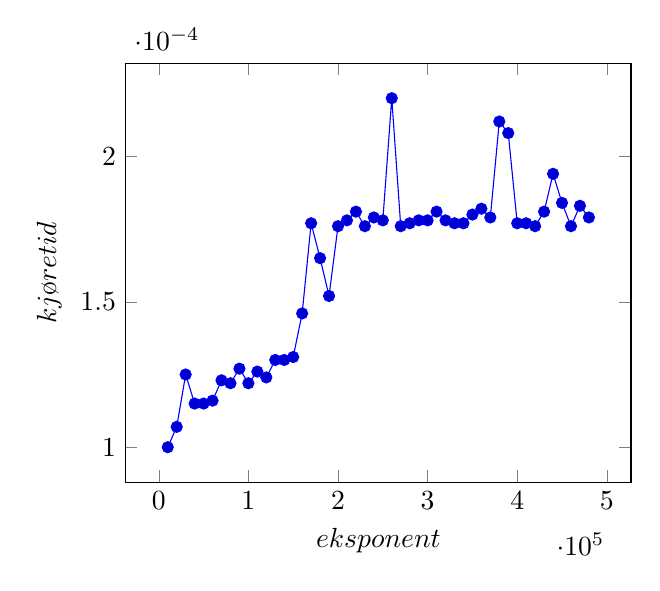
\begin{tikzpicture}
  \begin{axis}[
        xlabel = \(eksponent\),
        ylabel = {\(kjøretid\)},
  ]
    \addplot coordinates {
(10010, 0.000100)
(20010, 0.000107)
(30010, 0.000125)
(40010, 0.000115)
(50010, 0.000115)
(60010, 0.000116)
(70010, 0.000123)
(80010, 0.000122)
(90010, 0.000127)
(100010, 0.000122)
(110010, 0.000126)
(120010, 0.000124)
(130010, 0.000130)
(140010, 0.000130)
(150010, 0.000131)
(160010, 0.000146)
(170010, 0.000177)
(180010, 0.000165)
(190010, 0.000152)
(200010, 0.000176)
(210010, 0.000178)
(220010, 0.000181)
(230010, 0.000176)
(240010, 0.000179)
(250010, 0.000178)
(260010, 0.000220)
(270010, 0.000176)
(280010, 0.000177)
(290010, 0.000178)
(300010, 0.000178)
(310010, 0.000181)
(320010, 0.000178)
(330010, 0.000177)
(340010, 0.000177)
(350010, 0.000180)
(360010, 0.000182)
(370010, 0.000179)
(380010, 0.000212)
(390010, 0.000208)
(400010, 0.000177)
(410010, 0.000177)
(420010, 0.000176)
(430010, 0.000181)
(440010, 0.000194)
(450010, 0.000184)
(460010, 0.000176)
(470010, 0.000183)
(480010, 0.000179)
    };
  \end{axis}
\end{tikzpicture}
\end{center}

Grafen passer godt med grafen til funksjonen \(log(x)\)\\

Til slutt kan de sees ut som glibc sin pow funksjon operer i en konstant tid. Grafen viser eksponenten gå fra \(n = 10.000\) til \(n = 1.000.000\) med \(1.000\) som inkrement.

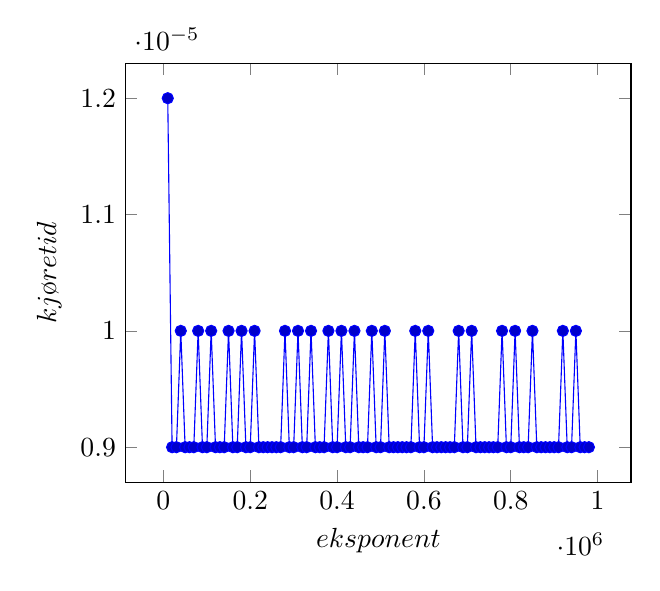
\begin{tikzpicture}
  \begin{axis}[
        xlabel = \(eksponent\),
        ylabel = {\(kjøretid\)},
  ]
    \addplot coordinates {
(10000, 0.000012)
(20000, 0.000009)
(30000, 0.000009)
(40000, 0.000010)
(50000, 0.000009)
(60000, 0.000009)
(70000, 0.000009)
(80000, 0.000010)
(90000, 0.000009)
(100000, 0.000009)
(110000, 0.000010)
(120000, 0.000009)
(130000, 0.000009)
(140000, 0.000009)
(150000, 0.000010)
(160000, 0.000009)
(170000, 0.000009)
(180000, 0.000010)
(190000, 0.000009)
(200000, 0.000009)
(210000, 0.000010)
(220000, 0.000009)
(230000, 0.000009)
(240000, 0.000009)
(250000, 0.000009)
(260000, 0.000009)
(270000, 0.000009)
(280000, 0.000010)
(290000, 0.000009)
(300000, 0.000009)
(310000, 0.000010)
(320000, 0.000009)
(330000, 0.000009)
(340000, 0.000010)
(350000, 0.000009)
(360000, 0.000009)
(370000, 0.000009)
(380000, 0.000010)
(390000, 0.000009)
(400000, 0.000009)
(410000, 0.000010)
(420000, 0.000009)
(430000, 0.000009)
(440000, 0.000010)
(450000, 0.000009)
(460000, 0.000009)
(470000, 0.000009)
(480000, 0.000010)
(490000, 0.000009)
(500000, 0.000009)
(510000, 0.000010)
(520000, 0.000009)
(530000, 0.000009)
(540000, 0.000009)
(550000, 0.000009)
(560000, 0.000009)
(570000, 0.000009)
(580000, 0.000010)
(590000, 0.000009)
(600000, 0.000009)
(610000, 0.000010)
(620000, 0.000009)
(630000, 0.000009)
(640000, 0.000009)
(650000, 0.000009)
(660000, 0.000009)
(670000, 0.000009)
(680000, 0.000010)
(690000, 0.000009)
(700000, 0.000009)
(710000, 0.000010)
(720000, 0.000009)
(730000, 0.000009)
(740000, 0.000009)
(750000, 0.000009)
(760000, 0.000009)
(770000, 0.000009)
(780000, 0.000010)
(790000, 0.000009)
(800000, 0.000009)
(810000, 0.000010)
(820000, 0.000009)
(830000, 0.000009)
(840000, 0.000009)
(850000, 0.000010)
(860000, 0.000009)
(870000, 0.000009)
(880000, 0.000009)
(890000, 0.000009)
(900000, 0.000009)
(910000, 0.000009)
(920000, 0.000010)
(930000, 0.000009)
(940000, 0.000009)
(950000, 0.000010)
(960000, 0.000009)
(970000, 0.000009)
(980000, 0.000009)
    };
  \end{axis}
\end{tikzpicture}

Resultatene tilsier at glibc sin pow funksjon opererer i konstant tid, og er dermed uavhengig av størrelsen på eksponenten, i motsetning til algoritmene implementert i denne øvingen.

\end{document}
